\documentclass[output=paper]{langsci/langscibook} 
\author{Ángel J. Gallego\affiliation{Universitat Autònoma de Barcelona}}
\title{Long distance agreement in Spanish dialects}

% \chapterDOI{} %will be filled in at production

% % \epigram{Change epigram in chapters/03.tex or remove it there }
\abstract{This paper discusses data from various dialects of Spanish manifesting agreement between an inflected verb and a \CATPP-internal \CATNP in the context of non-paradigmatic SE (e.g., Se vieron a los niños – Eng. ‘Children were seen’). An analysis is put forward in terms of Long Distance Agreement (cf. \citealt{Chomsky2000}; \citeyear{Chomsky2001Derivation}) between T (the locus of nominative Case) and an \CATNP Goal within a \CATKP/\CATPP. It is shown that this derivational possibility is subject to different microparametric layers teasing apart varieties allowing agreement across dative-like Case assigners (in differential object marking) and other prepositions that do not obviously participate in standard Case-agreement dependencies—thus giving rise to a pattern that qualifies as a pseudopassive of sorts.}
\maketitle

\begin{document}

 
%%please move the includegraphics inside the {figure} environment
%%\includegraphics[width=\textwidth]{OGSVolumeAug2018Gallego-img1.png}

 
%%please move the includegraphics inside the {figure} environment
%%\includegraphics[width=\textwidth]{OGSVolumeAug2018Gallego-img2.png}

 
%%please move the includegraphics inside the {figure} environment
%%\includegraphics[width=\textwidth]{OGSVolumeAug2018Gallego-img3.png}

 
%%please move the includegraphics inside the {figure} environment
%%\includegraphics[width=\textwidth]{OGSVolumeAug2018Gallego-img4}

 
%%please move the includegraphics inside the {figure} environment
%%\includegraphics[width=\textwidth]{OGSVolumeAug2018Gallego-img5}

 
%%please move the includegraphics inside the {figure} environment
%%\includegraphics[width=\textwidth]{OGSVolumeAug2018Gallego-img6}

 
%%please move the includegraphics inside the {figure} environment
%%\includegraphics[width=\textwidth]{OGSVolumeAug2018Gallego-img7}

 
%%please move the includegraphics inside the {figure} environment
%%\includegraphics[width=\textwidth]{OGSVolumeAug2018Gallego-img8}

 
%%please move the includegraphics inside the {figure} environment
%%\includegraphics[width=\textwidth]{OGSVolumeAug2018Gallego-img9.png}

 
%%please move the includegraphics inside the {figure} environment
%%\includegraphics[width=\textwidth]{OGSVolumeAug2018Gallego-img10}

 
%%please move the includegraphics inside the {figure} environment
%%\includegraphics[width=\textwidth]{OGSVolumeAug2018Gallego-img11}


\section{Introduction}% 1. 

It is an old observation that languages of the Spanish type fail to deploy both preposition stranding and pseudopassives, as the examples in (1) and (2) below show (cf. \citealt{Law2006} and references therein for discussion). 

\ea[*]{%1
    \label{ex:gallego:1}
    \langinfo{Spanish}{}{\citealt[741]{Campos1991}}\\
    \gll Quién contaron todos con?\\
           who    counted.\textsc{3pl}  all      with\\
    \glt  ‘Who did everybody count on?’}
    \z

\ea[*]{%2
    \label{ex:gallego:2}
    \langinfo{Spanish}{}{\citealt[741]{Campos1991}}\\
    \gll José es contado con   por todos.\\
         José be counted.\textsc{3sg} with by   everybody\\
    \glt ‘José is counted on by everybody.’}
    \z

Plausibly, the factor responsible for (1) is also behind (2), at least if the key element for both processes to take place is the category P, a locus of parametric variation (cf. \citealt{Hornstein1981,Kayne1984,Kayne1994,Kayne2005,Abels2003}; and references therein). In more abstract terms, we seem to be dealing with two constraints affecting prepositions and blocking both A and A-bar dependencies, which is what (3) is meant to capture:

\ea%3
    \label{ex:gallego:3}
     In the context Probe >>  \textbf{P}  >>  XP  ( >> = c-command)\\
     \begin{xlisti}\setcounter{xnumii}{1}
     \ex \ldots\xspace XP cannot move (no P-stranding)
     \ex \ldots\xspace XP cannot be a Goal (no pseudopassives)
     \end{xlisti}
\z

This paper discusses data from certain dialects of Spanish that depart from (3) in the context of passive SE sentences, at least for agreement cases. In particular, it will be shown that Long Distance Agreement (LDA) is possible between T (the locus of Nominative Case; cf. \citealt{Chomsky2000,Chomsky2001Derivation}) and a \CATDP Goal within a \CATPP. I will compare the data with previously reported evidence involving the Differential Object Marking preposition \textit{a} (cf. \citealt{Torrego1998,López2012}) in order to argue that there are three types of prepositions when it comes to the possibility for external Probes ($\varphi $-complete T) to bypass them.

The paper is organized as follows. §2 reviews the agreement options of passive SE sentences. §3 discusses the main properties of two patterns where T can agree with a \CATDP introduced by a preposition; the first pattern covers what \citet{RAE-ASALE2009} dubs the ‘hybrid pattern’ (agreement across the differential marker \textit{a}), whereas the second pattern involves agreement in the context of more full-fledged prepositions; §4 puts forward a Probe-Goal analysis of the facts (cf. \citealt{Chomsky2000,Chomsky2001Derivation}) that makes use of the idea that P can undergo incorporation (cf. \citealt{Hornstein1981,Law2006}). §5 contains the main conclusions.

\section{Agreement properties of SE sentences in Spanish}% 2. 

Passive\slash impersonal SE sentences have been the focus of much research (cf. \citealt{Mendikoetxea1992,Mendikoetxea1999,Raposo1996,D’Alessandro2007,López2007}; among others). If we concentrate on Spanish, it has been noted that the clitic SE can be part of structures where T agrees with the internal argument (IA, henceforth) (so-called Passive SE; see (4)), but it can also be part of structures where agreement fails (so-called Impersonal SE; see (5)), where T shows default agreement and the IA may or may not be headed by a Case marker, which depends on independent factors:

\ea%4
    Spanish\label{ex:gallego:4}\\
    \gll Se  criticaron        los recortes.        \\
         \textsc{se} criticize.\textsc{3pl}  the cuts\\
    \glt ‘Budget cuts were criticized.’
    \z

\ea%5
    Spanish\label{ex:gallego:5}\\
    \ea
    \gll Se   criticó             los  recortes.      \\
          \textsc{se}  criticize.\textsc{3sg}  the  cuts\\
    \glt ‘Budget cuts were criticized.’
    \ex
    \gll Se  criticó             a        los  políticos.           \\
         \textsc{se}  criticize.\textsc{3sg}  \textsc{dom} the politicians\\
    \glt ‘Politicians were criticized.’
    \z
\z

Consider the patterns above. The sentence in (4) contains a $\varphi $-defective \textit{v} that cannot Case-license the IA \textit{los recortes} (Eng. ‘the budget cuts’). As argued by both \citet{Raposo1996}, SE may be taken to occupy the external argument position (cf. \citealt{López2007}), thus behaving like an expletive of sorts (an idea that has been applied to spurious SE in clitic combinations; cf. \citealt[160]{Kayne2000}; \citealt{Gallego2017}). The sentences in (5) are not \textit{bona fide} passives: in such cases, \textit{v} is presumably $\varphi $-complete, and the IA receives accusative Case, which can be differentially marked (as in (5b)) or not (as in (5a)); as expected, T shows defective (3\textsuperscript{rd} person singular) agreement.

The two agreeing patterns of sentences involving SE have also been reported in traditional atlases such as the ALPI (Atlas Lingüístico de la Península Ibérica). The following data, taken from \citet{Benito2010}, show this:\footnote{Just to address a question by an anonymous reviewer, although the ALPI also collects information from Portugal, here I am focusing on Spanish data alone.} 

\ea%6
    (\citealt{Benito2010}: 8, 14)
    \label{ex:gallego:6}\\
    \ea Se \textbf{cortaron treinta pinos}. (Eng. ‘Thirty pines were cut.’)\\
        \todo[inline]{Note from the editor: The image is missing while we sort the licensing issues.}
          %%please move the includegraphics inside the {figure} environment
          %%\includegraphics[width=\textwidth]{OGSVolumeAug2018Gallego-img12.png}
    \ex Se \textbf{castigó} a \textbf{los ladrones} (Eng. ‘Thieves were punished.’)\\
    \todo[inline]{Note from the editor: The image is missing while we sort the licensing issues.}
          %%please move the includegraphics inside the {figure} environment
          %%\includegraphics[width=\textwidth]{OGSVolumeAug2018Gallego-img13.png}
    \z
\z

As a closer look at the data in (4) and (5) reveals, passive and impersonal SE sentences have a common base – they have the same argument structure, the only difference being agreement. In this context, \citet[§26.3.2.2]{Mendikoetxea1999} observes that passive SE sentences can manifest full or partial (defective) agreement, as illustrated in (7a) and (7b) respectively (cf. \citealt{Martín1979} for discussion):

\ea%7
    Spanish\label{ex:gallego:7}\\
    \ea
    \gll En  este  país        se   dicen       muchas  gilipolleces.       \\
         in   this   country  \textsc{se}  say\textsc{{}.3pl}  many     bullshit\\
    \glt ‘People say bullshit in this country.’
    \ex
    \gll En  este  país        se   dice        muchas  gilipolleces.       \\
         in   this   country  \textsc{se} say\textsc{{}.3sg}  many     bullshit \\
    \glt ‘People say bullshit in this country.’
    \z
\z

Although (7a) is clearly better to my ear, the patterns in (7) are both possible, and there is no consistent dialectal tendency, as far as I can tell. The $\varphi $-defective configuration has been reported in Old Spanish texts, and it is also present in varieties of present-day European and American Spanish (cf. \citealt{Mendikoetxea1999}).\footnote{\citet{RAE-ASALE2009} discusses a series of factors that may be behind the lack of agreement in such cases (the category of the internal argument, its preverbal\slash postverbal position, the presence of dative arguments, etc.). I put these issues aside here.} The $\varphi $-complete configuration involves unproblematic local agreement between T and the IA – a situation also displayed in \DAT-\NOM structures, whose intricacies I put aside here (cf. \citealt{López2007,Chomsky2008}).\footnote{An anonymous reviewer points out that we should not forget about discourse features and their valuation, as these are key in \DAT-\NOM constructions. It is unclear what the reviewer means here. If he\slash she is referring to notions like topic or focus, I simply do not assume they are features in the Probe-Goal sense (for discussion, see \citealt{Chomsky2001Derivation,Chomsky2008,Chomsky2017,Ott2016}). The fact that IOs participate in an agreement relation before DOs (or internal arguments more generally)  can be accounted for without resorting to any discourse feature.} 

There are more interesting cross-clausal cases, where agreement takes place at a distance. Thus, matrix T can long-distance agree with the IA of an embedded infinitive. This is well-known in the case of auxiliaries, but the pattern covers semi-auxiliaries and other verbs: 

\ea%8
\settowidth\jamwidth{[\textsc{semiaux} = try, need, etc.]}
    \label{ex:gallego:8}
    \ea\relax [ T [ SE  V\textsubscript{AUX}         [ INF XP ] ] ]      \jambox{[\textsc{aux} = can, should, etc.]}
    \ex\relax [ T [ SE  V\textsubscript{SEMIAUX}  [ INF XP ] ] ]         \jambox{[\textsc{semiaux} = try, need, etc.]}
    \z
\z    

Consider the following \citep[Chapter~28]{RAE-ASALE2009}, where I indicate Probe and Goal (the agreeing elements) with bold letters.

\ea%9
    Spanish\label{ex:gallego:9}\\
    \ea
    \gll Se  \textbf{intentan}  [ eliminar        \textbf{ciertas}  \textbf{leyes} ].        \\
         \textsc{se} tried\textsc{{}.3pl} {}  eliminate.\textsc{inf}  certain   laws\\
    \glt ‘Certain laws are tried to be eliminated.’  
    \ex
    \gll Se  \textbf{necesitan}  [ conocer     \textbf{sus}    \textbf{propiedades} ].         \\
            \textsc{se}  need\textsc{{}.3pl} {}  know.\textsc{inf}   their  properties\\
    \glt    ‘Their properties are needed to be known.’
    \ex
    \gll No se   \textbf{supieron}  [ usar        \textbf{esos}    \textbf{recursos} ].        \\
            not \textsc{se} knew\textsc{{}.3pl} {}   use.\textsc{inf}   those   resources\\
    \glt    ‘Those resources were not known to be used.’
    \ex
    \gll  Se   \textbf{han}           querido [ manchar        \textbf{reputaciones} ].     \\
            \textsc{se} have\textsc{{}.3pl} wanted {}   damage.\textsc{inf}   reputations\\
    \glt     ‘Reputations were wanted to be damaged.’
    \z
\z

Evidence like that provided by \citet{RAE-ASALE2009} has also been collected by dialectologists working on atlases:

\ea%10 
\gll En el huerto se \textbf{podían} plantar \textbf{rosales}.\\
in the garden \textsc{se} could.\textsc{3pl} plant rose.bushes\\
\glt ‘Rose bushes can be planted in the garden.’\\
(from \citealt[13]{Benito2010}) \\
     %%please move the includegraphics inside the {figure} environment
     %%\includegraphics[width=\textwidth]{OGSVolumeAug2018Gallego-img14.png}
\z

Interestingly, LDA situations go beyond SE scenarios, as shown in (11). As before, the $\varphi $-Probe on T scans into the embedded clause, displaying a phenomenon we can dub “hyperagreement”.\footnote{\citet{Fernández-Serrano2016} provides a detailed analysis of the data above based on the idea that agreement takes place whenever the embedded clause projects fewer layers of structure (undergoing a restructuring of sorts, but from a phase-theoretic perspective; cf. \citealt{Gallego2009}), which has morphological and interpretive consequences.} 

\ea%11
    \label{ex:gallego:11}
    \ea
    \gll Siempre   nos    \textbf{tocaron}              [ resolver  \textbf{problemas} ].\\
         always    to.us  be.our.turn.\textsc{3pl} {} solve       problems\\
    \glt ‘We always had to solve problems.’
    \ex
    \gll Nos   \textbf{faltan}    [ hacer  \textbf{dos}  \textbf{goles} ].\\
         to.us  lack.\textsc{3pl} {} make two goals\\
    \glt ‘We still have to score two goals.’
    \z
\z    

Notice that, in both SE and SE-less cases, agreement is only in number, not person (cf. \citealt{Etxepare2006}), but there seems to be robust evidence that we are dealing with syntactic LDA.\footnote{%
    A reviewer suggests that agreement is also for third person here, but this is not accurate, as this is a default value. If agreement was complete (number and person), then one would expect to find, for instance, SE sentences with 1st or 2nd person agreement; however, as \citet{López2007} points out, this is impossible in Spanish:
    
    \ea Spanish \citep[127]{López2007}\\
    \ea[*]{\gll Se  vimos      unos  lingüistas en  el   mercado ayer.\\
                \textsc{se}     saw.\textsc{1pl}  some linguists   in  the market    yesterday\\
           \glt ‘Some linguists were seen in the market yesterday.’\\(intended meaning: Some of us linguists were seen in the market)}
    \ex[*]{\gll Se  visteis      unos  lingüistas en  el    mercado  ayer.\\
                \textsc{se}  saw.\textsc{2pl}  some linguists   in  the  market     yesterday\\
            \glt ‘Some linguists were seen in the market yesterday.’\\(intended meaning: Some of you linguists were seen in the market)}
    \z
    \z} 
To conclude, consider previously unnoticed situations in which intervention-like effects arise in the context of an auxiliary: 

\ea%12
\judgewidth{?*}
    \label{ex:gallego:12}
    \ea[?]{
    \gll Me       \textbf{faltaron}      [ corregir \textbf{esos}   \textbf{exámenes} ].\\
         to.me   lacked.\textsc{3pl} {}  mark      those exams\\
    \glt ‘I couldn’t mark those exams.’}
    \ex[?*]{
    \gll Me      \textbf{faltaron}   [ haber  corregido \textbf{esos}    \textbf{exámenes} ].\\
         to.me  lacked\textsc{{}.3pl} {} have   marked     those  exams\\
    \glt ‘I couldn’t have marked those exams.’}
    \z
\z

A second piece of evidence comes from clitic climbing (cf. \citealt{Gallego2016,Paradís2016}; and references therein). As (13) shows, LDA is worse if a clitic stays in situ:

\ea%13
    \label{ex:gallego:13}
    \ea
    \gll Se  \textbf{pueden}  [ leer   \textbf{esos}    \textbf{libros} ].\\
         \textsc{se} can\textsc{{}.3pl} {}  read  those  books\\
    \glt ‘Those books can be read.’
    \ex
    \gll Se   (me)      \textbf{pueden}  [ leer(?*me)    \textbf{esos}    \textbf{libros} ].\\
         \textsc{se} to.me  can\textsc{{}.3pl} {}   {read   to.me}  those  books\\
    \glt ‘Those books can be read to me.’
    \z
\z

Let us conclude. This section has reviewed the main properties of SE sentences in Spanish, paying attention to the various agreement patterns they display in the different varieties of Spanish. Two main patterns have been identified, following the literature. One features a $\varphi $-defective \textit{v}, which explains the lack of accusative Case (and thus agreement with T). The other features a $\varphi $-complete \textit{v}, which blocks Agree (T, IA). As we have seen, the alternation between agreeing and non-agreeing options is not subject to any systematic dialectal logic (there is no “isogloss” telling us where agreement stops), so we seem to have a case of optionality – with a tendency towards full agreement, a murky issue that seems to have semantic consequences in biclausal scenarios (cf. \citealt{Martin1998,Fernández-Serrano2016}). 

As we have seen, such optionality is frequent whenever the IA is not differentially marked. However, agreement has also been reported in cases where the DO is preceded by a Case marker, a pattern I would like to refer to as hybrid, which I discuss in the following section.

\section{Agreement across P in Spanish} % 3. 
\subsection{Introduction}%  3.1. 

This section considers two configurations in which agreement between T and the complement of a preposition can take place in Spanish. The first one involves the differential marker \textit{a} (cf. \citealt{Torrego1998,López2012}) and the second one involves full-fledged prepositions. Roughly, the relevant abstract patterns are as in (14), where K and P give rise to Case and P projections.\footnote{The distinction between K and P is equivalent to that between functional or lexical prepositions (see \citealt{Riemsdijk1990} and references therein for discussion).}

\ea%14
    \label{ex:gallego:14}
    \ea\relax [ SE \ConnectTail{\textbf{T}} (Probe)  [\textsubscript{VP} V \ldots\xspace [ K \ConnectHead[1.5ex]{\textbf{XP}} (Goal)\,]\,]\,]  [K = differential marker]
    \vspace{\baselineskip}
    \ex\relax [ SE \ConnectTail{\textbf{T}} (Probe)  [\textsubscript{VP} V \ldots\xspace [ P \ConnectHead[1.5ex]{\textbf{XP}} (Goal)\,]\,]\,]  [P = full-fledged preposition]
    \z
\z


%%please move the includegraphics inside the {figure} environment
%%\includegraphics[width=\textwidth]{OGSVolumeAug2018Gallego-img15}
 
%%please move the includegraphics inside the {figure} environment
%%\includegraphics[width=\textwidth]{OGSVolumeAug2018Gallego-img16}

After briefly discussing the case of agreement across \DOM (namely, (14a)), I turn my attention to (14b), suggesting that P undergoes incorporation, giving rise to a P-stranding-less version of pseudopassives. In terms of parametric tendencies, the second scenario is unexpected, given the properties of Romance languages. This should explain its limited availability, which seems to be largely restricted to American varieties.

\subsection{Agreement across \DOM}% 3.2. 

We have already seen that SE sentences can be passive (with agreement) and impersonal (without agreement). Above we saw the relevant data in (4) and (5), repeated as (15) and (16):

\ea%15
    Spanish\label{ex:gallego:15}\\
    \gll Se  criticaron        los recortes.            \\
         \textsc{se} criticize\textsc{{}.3pl}  the cuts\\
    \glt ‘Budget cuts were criticized.’
    \z  

\ea%16
    Spanish\label{ex:gallego:16}\\
    \ea
    \gll Se   criticó             los  recortes.            \\
         \textsc{se} criticize\textsc{{}.3sg}  the  cuts\\
    \glt ‘Budget cuts were criticized.’
    \ex
    \gll Se  criticó             a        los  políticos.\\
         \textsc{se} criticize\textsc{{}.3sg}  \textsc{dom} the politicians\\
    \glt ‘Politicians were criticized.’
    \z
\z

As noted, if \textit{v} is $\varphi $-complete (the (15) example), the IA presumably receives accusative Case, which can be coupled with the differential marker \textit{a}, as in (16b). This is precisely the pattern in which agreement is most unlikely to happen – for the same reason agreement does not bypass prepositions more generally. That said, agreement does seem to be possible in some cases, even in the context of \DOM; this variant of the pattern in (16b), to which I return below, is called “hybrid” by \citet{RAE-ASALE2009}.\footnote{Variation in this domain does not seem to adhere to any clear-cut geographical distinction. For some speakers, agreement is optional, and has no interpretive consequences. \citet{Planells2017} approaches the facts by taking T to agree optionally with SE or the (shifted, for \DOM reasons) internal argument – which are responsible for partial and complete agreement respectively. The approach makes use of \citegen{Chomsky1995} \textit{equidistance} (cf. \citealt{Gallego2013} for discussion), but the facts could also be handled by the approach to variation put forward in \citet{Obata2016}, where parameters boil down to SMT-compliant derivations whose order of operations varies.}

The \textit{v} of (16) should be $\varphi $-complete \textit{v}, therefore \textit{v}* in the sense of \citet{Chomsky2001Derivation}. However, it is not immediately obvious that \textit{bona fide} Accusative Case is assigned in the two examples offered in (16). Consider the contrast in (17), where the accusative clitic \textit{lo} (Eng. ‘it’) can only be used if the antecedent is animate (\textit{a Trump} – Eng. ‘Trump’):\footnote{As an anonymous reviewer rightly points out, there is non-trivial variation concerning the case of clitics in these constructions, even within European varieties of Spanish. Taking into account all the dialectal subtleties that concern clitics is beyond the scope of this paper.}

\ea%17
    \label{ex:gallego:17}
    \ea[*]{
    \gll Los poemas, se   \textbf{los}                recita        en clase de literatura.            \\
         the  poems   \textsc{se} it\textsc{{}.acc}.\textsc{m.pl} read\textsc{{}.3}\textsc{sg}  in  class of literature\\
    \glt ‘Poems, we read them in literature class.’}
    \ex[?]{
    \gll A Trump,  aquí  se   \textbf{lo}                   ve           como a   un matón.   \\
         \textsc{dom} Trump   here  \textsc{se} it\textsc{{}.acc}.\textsc{m.sg} see\textsc{{}.3}\textsc{sg} like    to  a    thug\\
    \glt ‘Trump, he is seen as a thug here.’   }
    \z
\z   

The asymmetry in (17) looks consistent, so let’s assume the following generalization, taking it for granted that only \DOM signals Accusative Case assignment:\footnote{Although (18) is stable across dialects, there are well-known exceptions. In particular, the pattern is more restricted in European Spanish. In non-European varieties, on the other hand, \citet[§41.12m]{RAE-ASALE2009} observes that \textit{v}* can assign Accusative Case to inanimate IAs in the Andean, Chilean, and River Plate areas (cf. \citealt{Gallego2016}).}

\ea%18
\label{ex:gallego:18}
If the IA is differentially-marked (\textit{a} XP), then SE \textit{v} is \textit{v}* ($\varphi $-complete).
\z

          

An interesting piece of evidence indicating that accusative Case may not be at play even in the presence of \DOM comes from the observation that leísta varieties of Spanish show a preference for the dative clitic \textit{le} (Eng. ‘to him\slash her’) in the presence of SE, as in (19):

\ea%19
    \ea
    Non-leísta/American Spanish\label{ex:gallego:19}\\
    \gll Se  \textbf{lo}       critica.          \\
              \textsc{se}  \textsc{cl.acc} criticize\textsc{{}.3}\textsc{sg}\\
    \glt      ‘He is criticized.’
    \ex Leísta/European Spanish\\
    \gll Se \{?\textbf{lo}    /    \textbf{le}\}       critica.      \\
                 \textsc{se}   \textsc{cl.acc} ~ \textsc{cl.dat}   criticize\textsc{{}.3}\textsc{sg}\\
    \glt      ‘He is criticized.’
    \z
\z   

This raises the more general question whether differentially-marked IAs receive true accusative. If the answer is negative, this would explain the restricted availability of \textit{lo}/\textit{la} (only with animates), and the preference for \textit{le} in European Spanish. The tendency to have a \textit{lo > le} shift in the context of SE is noted by \citet{Ordóñez2004}:

\ea%20
    European Spanish\label{ex:gallego:20}\\
    \gll Si hay                 que  fusilar-\textbf{lo},  SE \textbf{le} fusila.\\
        if  there.be\textsc{{}.3}\textsc{sg}  that  shoot\textsc{{}-cl}  \textsc{se}  \textsc{cl}  shoot\textsc{{}.3}\textsc{sg}\\
    \glt ‘If he must be shot, he is shot.’ (from P. Preston, \textit{Franco}, cited by \citealt{Ordóñez2004})
    \z

This accusative-dative connection would naturally align with leísmo, which seems to be present in the only Romance language with consistent \DOM: Spanish. \citet{Colomina2017} in fact argue that \DOM involves a process of accusative Case displacement, assuming that the structure that underlies (21) is (22):

\ea%21
    Spanish\label{ex:gallego:21}\\
    \gll Nadie    visitó             a          Trump.   \\
         nobody  visited\textsc{{}.3}\textsc{sg}  \textsc{dom}   Trump\\
    \glt ‘Nobody visited Trump.’
    \z

\ea%22
    \label{ex:gallego:22}
    [\textit{\textsubscript{v}}\textsubscript{P} nadie \textit{v} [\textsubscript{VP} PROVIDE [ (to) Trump [ P VISIT ] ] ] ]
\z

          

In this context, it is interesting to note that Mexican Spanish, which is not leísta, becomes (obligatorily) leísta if SE is introduced. In fact, as (23) reveals, this type of leísmo is more general than the one present in European varieties, for it applies to both masculine and feminine {\CATDP}s (as in \textit{bona fide} datives, as emphasized by \citealt{Colomina2017}).

\ea%23
    Mexican Spanish\label{ex:gallego:23}\\
    \ea
    \gll A       tu      amigo         SE  \textbf{le} ve         preocupado.  \\
         \textsc{dom}   your friend\textsc{{}.m.}\textsc{sg} \textsc{se}   him\textsc{{}.dat.m.}\textsc{sg}  see\textsc{.3sg} worried\\
    \glt ‘Your friend, he looks worried.’
    \ex
    \gll A       tu      amiga        SE  \textbf{le} ve          preocupada. \\
         \textsc{dom}   your friend\textsc{{}.f.}\textsc{sg} \textsc{se}   her\textsc{{}.dat.f.}\textsc{sg} see\textsc{.3sg} worried\\
    \glt ‘Your friend, she looks worried.’
    \z
\z

\citet{Gallego2016} builds on the previous description of the facts to argue that impersonal SE sentences can be divided into two broad dialects:

\ea%24
    \label{ex:gallego:24}
    \ea Dialect A: \textit{v} is $\varphi ${}-defective
    \ex Dialect B: \textit{v} is $\varphi ${}-complete
    \z
\z

The morphological distinction targeting \textit{v} implies the following:

\ea%25
    \label{ex:gallego:25}
    \ea Leísta Spanish\\
     Dialect A:   [\textit{\textsubscript{v}}\textsubscript{P} \textit{v} [\textsubscript{VP} V  [\textsubscript{PP} \ConnectTail{\textit{a}}   [ \ConnectHead{DP}\textsubscript{OBLIQUE}] ] ] ] 
    \ex Non-leísta Spanish\\
    Dialect B:  i.  [\textit{\textsubscript{v}}\textsubscript{P} \ConnectTail{\textit{v}$\varphi $} [\textsubscript{VP} V [\textsubscript{KP} \textit{a} \ConnectHead{DP}\textsubscript{ACC} ] ] ]
    \ex Hybrid pattern\\
    Dialect B:  ii.   [ \ldots\xspace \ConnectTail{T$\varphi $} \ldots\xspace [\textit{\textsubscript{v}}\textsubscript{P} \textit{v} [\textsubscript{VP} V [\textsubscript{KP} \textit{a} \ConnectHead{DP}\textsubscript{NOM} ] ] ] ]
    \z
\z    

%%please move the includegraphics inside the {figure} environment
%%\includegraphics[width=\textwidth]{OGSVolumeAug2018Gallego-img17}
%%please move the includegraphics inside the {figure} environment
%%\includegraphics[width=\textwidth]{OGSVolumeAug2018Gallego-img18}
% %%please move the includegraphics inside the {figure} environment
% %%\includegraphics[width=\textwidth]{OGSVolumeAug2018Gallego-img19}


The key distinction between A and B dialects is whether Accusative Case is assigned or displaced. If the latter is the case, some oblique (dative, if some version of \citegen{Marantz1991} Dependent Case approach is at work) assigner takes care of the IA.

The most intriguing pattern is (25c), which is reported by \citet{Ordóñez2007}. As these authors note, Mexican and Argentinian varieties of Spanish feature what \citet{RAE-ASALE2009} calls the ‘hybrid’ pattern (cf. \citealt{Planells2017} and references therein for discussion).

\ea%26
    (\citealt[12]{Ordóñez2007})\\
    \ea Mexican Spanish\label{ex:gallego:26}\\
    \gll Finalmente, se  \textbf{castigaron}       a  \textbf{los} \textbf{culpables}.        \\
         finally         \textsc{se}   punished.\textsc{3pl}   to the culprits\\
    \glt ‘Finally, the culprits were punished.’
    \ex Argentinian Spanish\\
    \gll Se  \textbf{evacuaron}    a más de \textbf{120.000} \textbf{damnificados}.              \\
         \textsc{se}   evacuated.\textsc{3pl} to more of 120,000 damaged\\
    \glt  ‘More than 120,000 damaged people were evacuated.’
    \z
\z

These data are not expected if the IA is inactive, after receiving accusative Case. In order to account for them, we would need to assume that: (i) the IA is Case-less (otherwise the $\varphi $-Probe on T could not match it) and (ii) the Case marker \textit{a} cannot give rise to a \CATPP or a \CATKP projection. It must in fact be analyzed as an element inserted in the NS → PF wing of the derivation – in other words, as a dissociated morpheme (cf. \citealt{Halle1993}).

  Now that we have reviewed agreement across differential markers, in the next section I pay attention to situations where agreement is rampant, and in fact ignores elements that are not mere functional Case markers, but are seemingly full-fledged prepositions.

\subsection{Agreement across full-fledged P}% 3.3.

We have just discussed data where the $\varphi $-Probe on T within SE sentences matches a differentially marked IA. Such cases, though subject to a rather unclear dialectal distribution, fall into place if Spanish \textit{a} can be considered a functional element, not a preposition in its own right. Surprisingly, some American Spanish dialects seem to allow a pattern of agreement that can also ignore prepositions other than \textit{a}. Consider the examples in (27), taken from internet searches:

\ea%27
    American Spanish\label{ex:gallego:27}\\
    \ea
    \gll Dijo que se  \textbf{hablaron}    con   \textbf{las}   \textbf{autoridades}.\\
         said.\textsc{3sg}  that \textsc{se}   talked.\textsc{3pl}  with  the  authorities\\
    \glt ‘He said that the authorities were talked to.’\\
    {\small\url{http://www.santiagodigital.net/index.php?option=com\_content\& task=view\& id=13837\& Itemid=17}}
    \ex
    \gll En Santiago anoche    se  \textbf{informaron}   de \textbf{cuatro}  \textbf{homicidios}.\\
         in  Santiago {last night} \textsc{se}   informed.\textsc{3pl} of  four     homicides\\
    \glt ‘Four homicides were reported last night in Santiago.’\\
    {\small\url{http://www.periodismoglobal.cl/2006/08/la-democracia-de-la-udi.html}}
    \ex
    \gll El  comercio online sumó [...]   100 millones de transacciones.          [...] cuando se   \textbf{llegaron}       a   \textbf{los} \textbf{74,3} \textbf{millones}  \textbf{de} \textbf{operaciones}.\\
         the trade       online added{}.\textsc{3sg} {} 100 millions  of transactions {}               when    \textsc{se}   arrived{}.\textsc{3pl}  to the 74.3 millions    of operations\\
    \glt ‘The online trading added 100 million transactions when 74.3 million operations were reached.’\\
    {\small\url{http://www.elpais.com/articulo/economia/comercio/electronico/volvio/batir/record/2010/elpepueco/20110506elpepueco\_7/Tes}}
    \ex
    \gll En realidad se  \textbf{dependen} de  \textbf{tantos} \textbf{factores}  que  esto provoca  una extrema  dificultad\\
         in   reality   \textsc{se}   depend{}.\textsc{3pl} of   so.many    factors  that this provokes a    extreme  difficulty\\
    \glt ‘Actually, one depends on so many factors that it makes things extremely difficult.’\\
         {\small\url{http://diegotenis9.wordpress.com/}}
    \z
\z    

Analogous data can be obtained from searches in both the CREA data bank and on Google:



\ea%28
    (from CREA: http://corpus.rae.es/creanet.html)\label{ex:gallego:28}\\
    \ea  El Salvador\\
    \gll Sólo se  \textbf{disponen}     de  \textbf{datos} \textbf{de}  \textbf{matrículas} …     \\
         just  \textsc{se}   dispose{}.\textsc{3pl} of  data    of  registration\\
    \glt ‘We just have data on registration …’
    \ex  Costa Rica\\
    \gll Aunque   no   se \textbf{disponen}      de  \textbf{cifras}       \textbf{exactas} …  \\
         although not \textsc{se}   dispose{}.\textsc{3pl}  of   numbers  exact\\
    \glt ‘Although we don’t have exact numbers …’
    \ex  Spain\\
    \gll   Sí   se  \textbf{saben}        de \textbf{diversos} \textbf{factores} que influyen …  \\
           yes \textsc{se}   know{}.\textsc{3pl}  of  diverse   factors    that influence\\
    \glt   ‘We do know factors that influence …’
    \z
\z    


\ea%29
    \label{ex:gallego:29}
    \ea  Mexico\\
    \gll Todavía se   \textbf{confían}    en  los   milagros.\\
         yet         \textsc{se}   trust{}.\textsc{3pl}  in  the   miracles\\
    \glt ‘They still believe in miracles.’\\
    {\small\url{http://www.sinembargo.mx/30-03-2014/947521}}
    \ex  Chile\\
    \gll Cuando se   \textbf{hablan}    de  \textbf{las} \textbf{supuestas} \textbf{desigualdades} \\
         when     \textsc{se}   talk{}.\textsc{3pl}   of  the alleged      asymmetries\\
    \glt ‘When they talk about the alleged asymmetries’\\
    {\small\url{http://blog.lanacion.cl/2014/03/11/desigualdades-de-genero-en-el-emprendimiento/}}
    \z
\z    

These data have not been described in reference grammars of Spanish (cf. \citealt{Bosque1999,RAE-ASALE2009}), plausibly because they can be can be regarded as production errors. The data have, however, also been reported by the Syntactic Atlas of Spanish (ASinEs) (see \figref{ex:gallego:30}).

% % % \ea%30
\begin{figure}[t]\caption{Syntactic Atlas of Spanish. \citep{GallegoWebsite}\label{ex:gallego:30}}
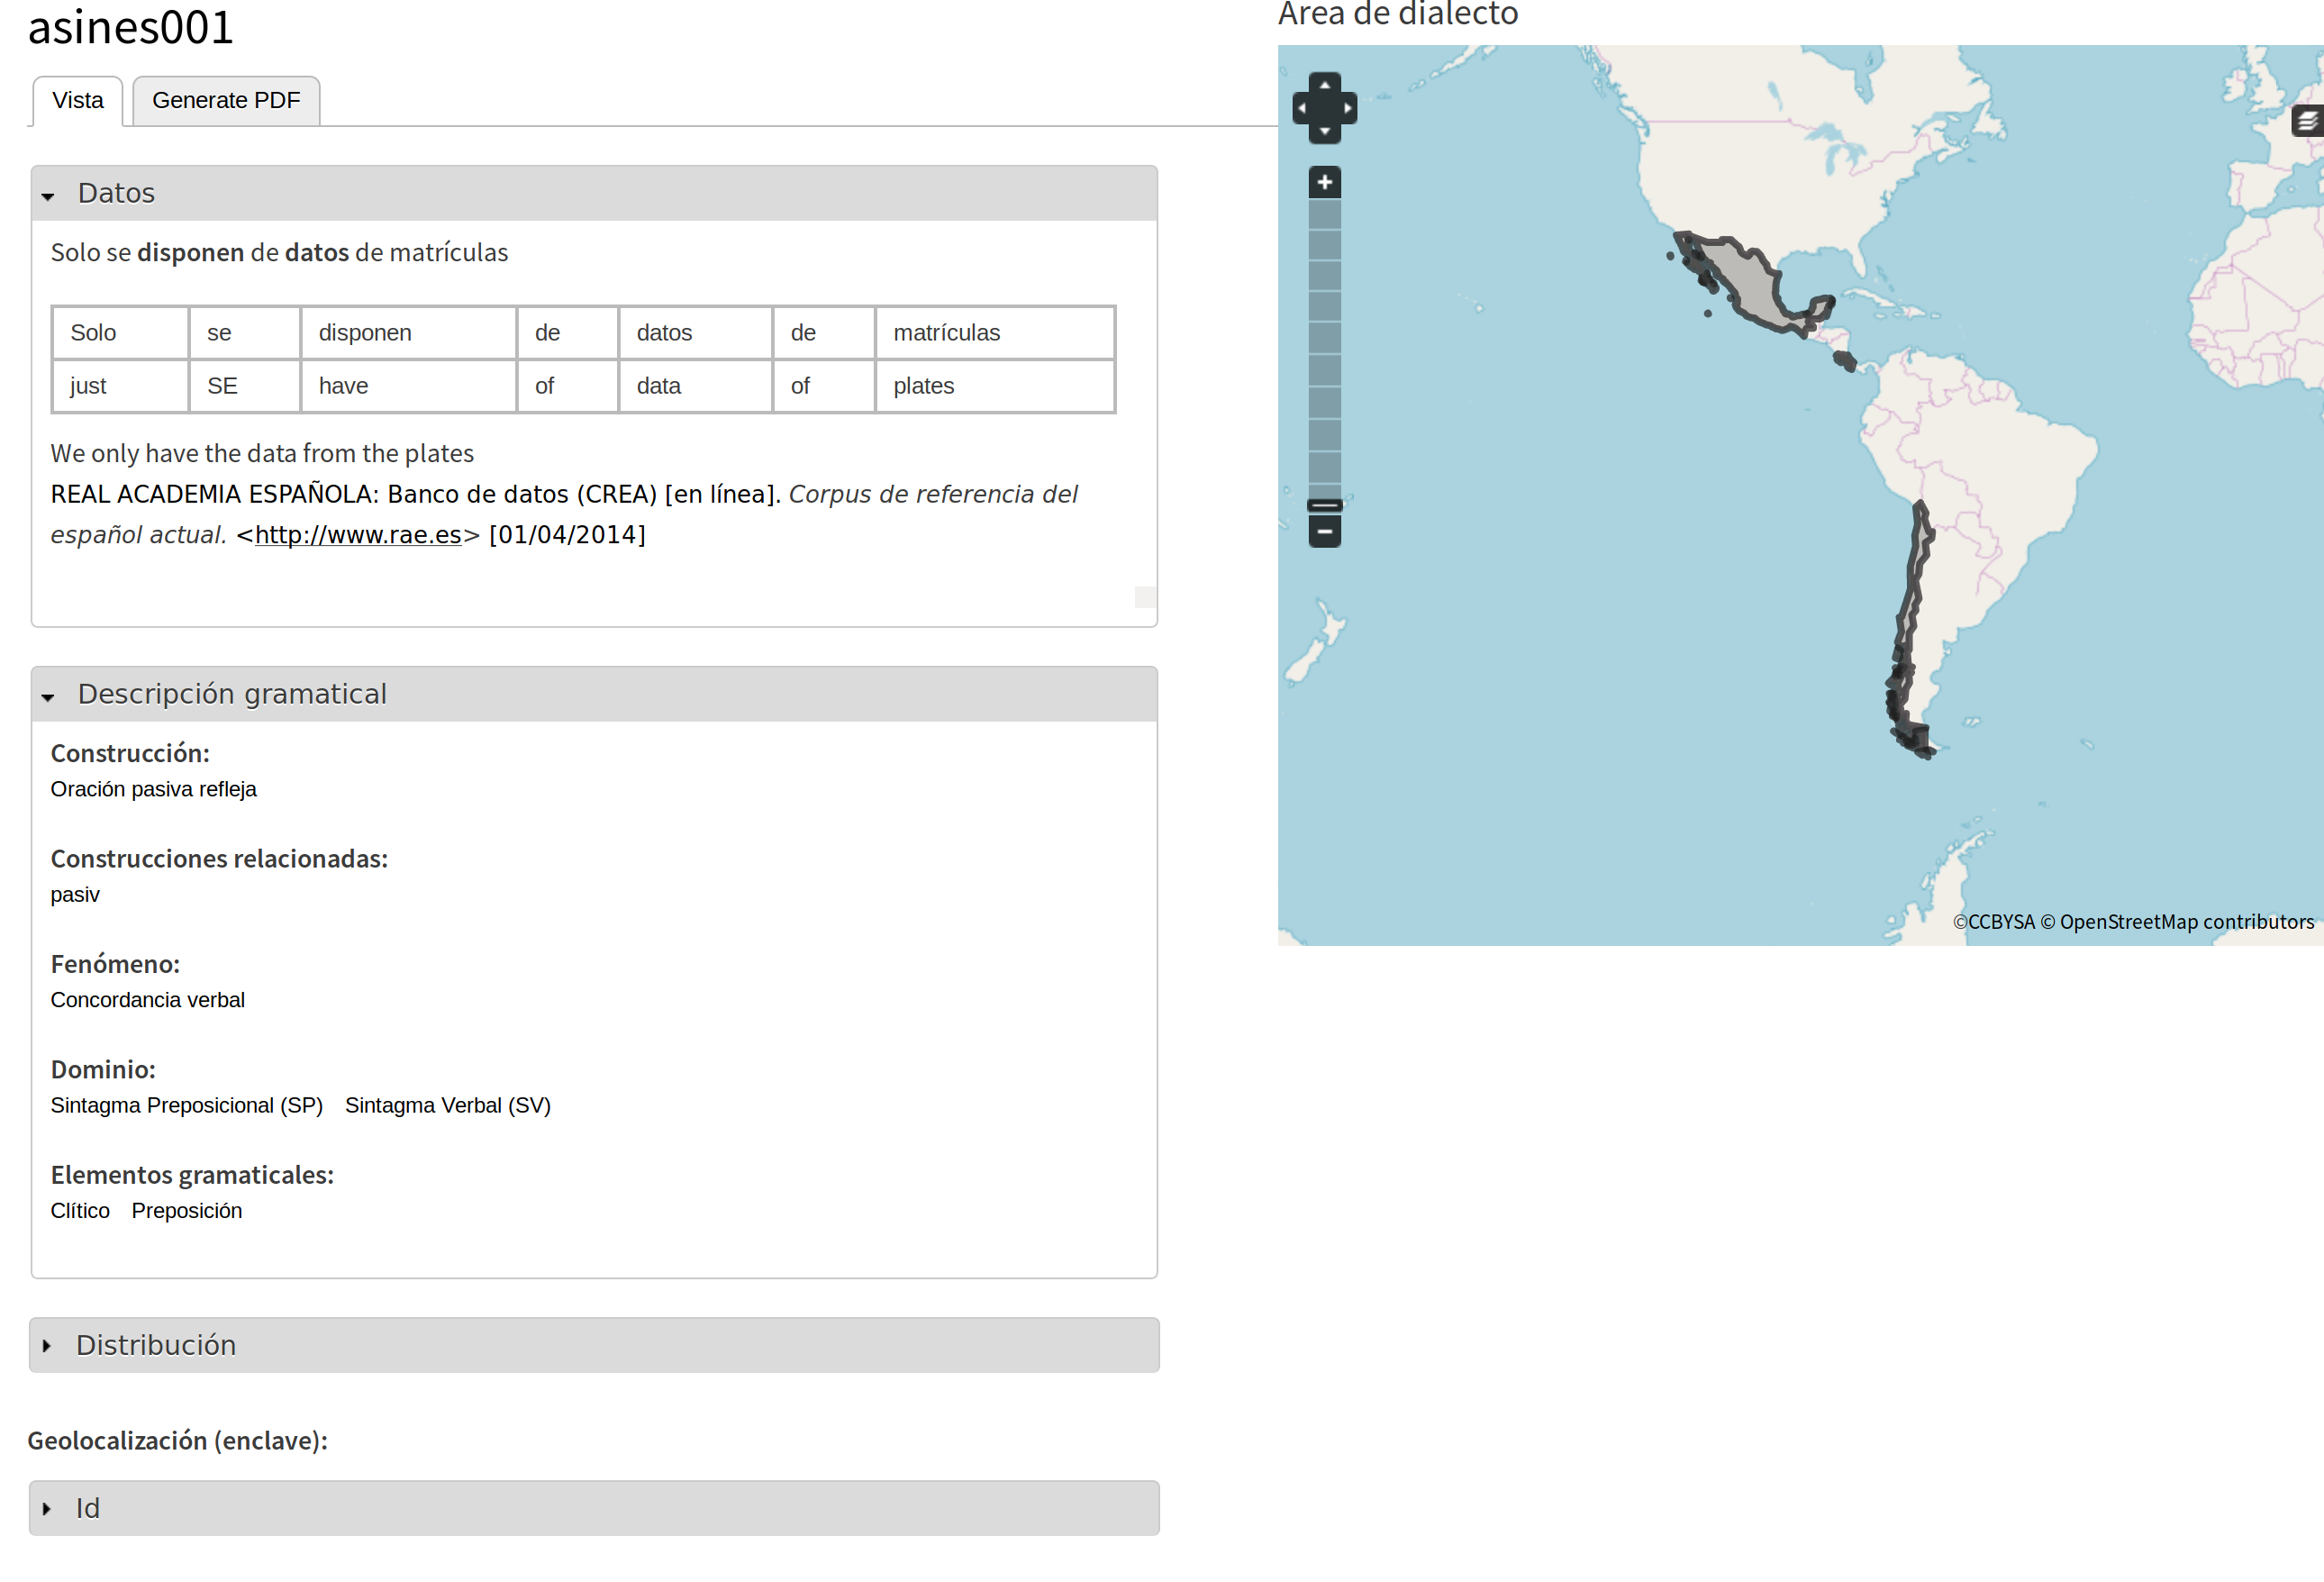
\includegraphics[width=\textwidth]{figures/gallego-screenshot.png}
\end{figure}


Furthermore, note that the texts from which I have gathered the examples are not oral, and they are not isolated online hits. The fact that this type of evidence can also be found in the CREA database seems to me enough to regard it as part of the speakers’ competence. Therefore, what one could plausibly conclude from these examples is that American dialects of Spanish display a restricted variety of pseudopassives (modulo P-stranding). Let us refer to this process as “P-phasing”, merely to indicate that the P undergoes a change of state that allows the $\varphi ${}-Probe on T to match the \CATDP. 

\section{A Probe-Goal analysis of the facts}% 4. 


Some questions arise if, as I have argued, the prepositions in the examples can be bypassed by a $\varphi ${}-Probe. To begin with, one may wonder whether the same phenomenon is found not only with SE passives, but also with periphrastic (BE) passives. The answer is negative, as examples like the following are ruled out by American Spanish speakers who accept the data in  (27), (28) and (29):



\ea%31
    American Spanish\label{ex:gallego:31}\\
    \ea[*]{
    \gll \textbf{Fueron}  \textbf{habladas}          con   \textbf{las}  \textbf{autoridades}.  \\
         be{}.\textsc{3pl}   talked{}.\textsc{f.3pl} with  the  authorities\\
    \glt ‘The authorities were spoken to.’  }
    \ex[*]{
    \gll  \textbf{Fueron}  \textbf{informados}              de  \textbf{cuatro} \textbf{homicidios}. \\
          be{}.\textsc{3pl}   informed.\textsc{m.3pl} of    four     homicides \\
    \glt  ‘Four homicides were reported.’
    }
    \z
\z    

The process of P-phasing might further be related to the prepositional-transitive alternation, illustrated in (31), that many prepositional verbs undergo in Spanish (cf. \citealt{Demonte1991,García-Miguel1995,Gallego2010}; and references therein):\footnote{Plausibly too, the speakers that allow for P-phasing also accept P-stranding in Spanish (cf. \citealt{Depiante2013,Lemos2013}; and references therein).}

\ea%32
    Spanish\label{ex:gallego:32}\\
    \ea
    \gll He             pensado (en) la     respuesta.        \\
         have{}.\textsc{1sg}  thought    in   the   answer\\
    \glt ‘I thought of the answer.’
    \ex
    \gll Hemos      discutido  (de)     ese  asunto  en  la   reunión.  \\
         have{}.\textsc{1pl}  discussed  about  that  matter  in  the meeting\\
    \glt ‘We discussed that matter in the meeting.’
    \z
\z

This very point takes us back to a second question posed by the data above. What is the relevant parameter that makes agreement possible across prepositions? I will assume that the T head is morphologically equivalent in all the Spanish dialects under consideration – hence, there is no parametrically ‘tweaked’ version of T that allows for a deeper search (cf. \citealt{Chomsky2001Derivation}). I will instead argue that it is the status of P that varies, as whatever happens in these dialects affects the \textit{v}P syntax. There are three specific alternatives to implement the idea that the parameter is anchored to P:

\ea%33
    Parametrizing P\label{ex:gallego:33}\\
    \ea P is external to the VP (as in \citeauthor{Kayne2004}'s 2004 analysis of causatives)
    \ex P is inserted at PF (as a dissociated morpheme)
    \ex P is reanalyzed with V
\z
\z

The first option is tempting in the case of the hybrid pattern, where the preposition has a clear-cut functional nature – like complementizers, as \citet{Kayne2004} argues. This is in fact the approach that \citet{Ordóñez2016} put forward in their analysis of \DOM, whose derivation is reproduced in (35) for a sentence like (34):

\ea%34
    Spanish\label{ex:gallego:34}\\
    \gll   Vimos     a          María.\\
           saw{}.\textsc{1pl}  \textsc{dom}   María\\
    \glt   ‘We saw María.’
\z
  
\ea
    \ea …  [\textit{\textsubscript{v}}\textsubscript{P}  \textit{v}  [\textsubscript{VP} vimos   [\textsubscript{DP} María ] ] ]    DP [+anim, +spec]\\
    Merge of \textit{a}
    \ex  …  a  [\textit{\textsubscript{v}}\textsubscript{P}  \textit{v}  [\textsubscript{VP} vimos   [\textsubscript{DP} María ] ] ]\\
    Movement to Spec 
    \ex  …  [\textit{\textsubscript{a}}\textsubscript{P} [María]\textsubscript{i}  a  [\textit{\textsubscript{v}}\textsubscript{P}  \textit{v}  [\textsubscript{VP} vimos [t]\textsubscript{i} ] ] ] \\
    Merge of W 
    \ex …  W [\textit{\textsubscript{a}}\textsubscript{P} [María]\textsubscript{i}  a  [\textit{\textsubscript{v}}\textsubscript{P}  \textit{v}  [\textsubscript{VP} vimos [t]\textsubscript{i} ] ] ]  \\
    Head raising 
    \ex …  [a\textsubscript{j}+W] [\textit{\textsubscript{a}}\textsubscript{P} [María]\textsubscript{i}  t\textsubscript{j}  [\textit{\textsubscript{v}}\textsubscript{P}  \textit{v}  [\textsubscript{VP} vimos [t]\textsubscript{i} ] ] ]  \\
    Remnant movement
    \ex …  [\textsubscript{WP}  [\textit{\textsubscript{v}}\textsubscript{P}  \textit{v}  [\textsubscript{VP} vimos [t]\textsubscript{i} ] ] ]\textsubscript{k} [a\textsubscript{j}+W] [\textit{\textsubscript{à}}\textsubscript{P} [María]\textsubscript{i}  t\textsubscript{j}  t\textsubscript{k}  
    \z
\z

Suppose that, following the logic of these authors’ analysis, the differential marker is introduced above the TP (not the \textit{v}P), then there is no obstacle preventing T’s $\varphi ${}-Probe from matching the IA. It is not obvious, though, that the same idea should be adopted for prepositions that have a semantic flavor, like many of those featured in the examples above. For this very reason, it is not obvious that the analysis in (34) can be phrased in terms of PF insertion: the prepositions in (27), (28) and (29) are not dissociated morphemes. We are left, therefore, with some variant of the reanalysis approach (cf. \citealt{Hornstein1981,Kayne1975,Kayne2004}, among many others). Of course, notice that it must be the case that the preposition is not heading an adjunct, since these seem to block agreement at all costs. Hence, the examples in (36) are totally out:



\ea%36
    Spanish\label{ex:gallego:36}\\
    \ea[*]{
    \gll Se  \textbf{trabajaron}  en  \textbf{las} \textbf{reuniones}.   \\
         \textsc{se}   work.\textsc{3pl}     in  the meetings\\
    \glt ‘People worked in the meetings.’  }
    \ex[*]{
    \gll Se   \textbf{criticaron}     al              Presidente  por \textbf{varias} \textbf{razones}. \\
         \textsc{se}   criticize.\textsc{3pl} \textsc{dom}{}-the president      for various reasons\\
    \glt ‘The President was criticized for various reasons.’  }
    \z
\z    

Consequently, the V-P reanalysis option seems to be necessary with some prepositions. Accordingly, the process depicted in (36) seems to be relevant for capturing the data in (27), (28) and (29):


\ea%37
    \label{ex:gallego:37}
    \ea\onehalfspacing\relax [ SE \ConnectTail{\textbf{T}} ($\varphi $-Probe)  [\textsubscript{VP} V \ldots\xspace [  P \ConnectHead{\textbf{XP}} (Goal) ] ] ] (P = full-fledged preposition) 
    \ex\onehalfspacing\relax [ SE \ConnectTail{\textbf{T}} ($\varphi $-Probe)  [\textsubscript{VP} [V-P] \ldots\xspace [ t  \ConnectHead{\textbf{XP}} (Goal) ] ] ] (P = full-fledged preposition)
    \z
\z
%%please move the includegraphics inside the {figure} environment
%%\includegraphics[width=\textwidth]{OGSVolumeAug2018Gallego-img21}

%%please move the includegraphics inside the {figure} environment
%%\includegraphics[width=\textwidth]{OGSVolumeAug2018Gallego-img22}

Literally, what (37) is saying is that P is incorporated into V so that the XP Goal is probeable by T and agreement can take place. This raises interesting typological questions of the sort involved in teasing apart satellite-framed and verb-framed languages (cf. \citealt{Mateu2012} and references therein). An observation to keep in mind in order to support the Probe-Goal analysis is that, again, agreement is only in number (cf. \citealt{Etxepare2006}), as the following asymmetries reveal:



\ea[*]{%38
         Spanish\label{ex:gallego:38}\nopagebreak\\
    \gll Se \{pensa-mos/-áis\}   en  \{nosotros / vosotros\}.      \\
         \textsc{se}   think-\textsc{1pl/-2pl}     in    we      /      you.\textsc{pl}\\
    \glt ‘We/you are thought about.’ }
    \z
    
Finally, there is evidence arguing against the existence of a non-referential (indefinite) \textsc{3pl} pronoun (cf. \citealt{Suñer1983,Cabredo2003}). These pronouns can be spelled out, and then the non-referential reading is lost. However, these sentences reject the spell-out of a pronoun. So, the following is possible:

\ea%39
    Spain\label{ex:gallego:39}\\
    \gll En España, (ellos)  se  acuestan            tarde.    \\
         in  Spain       they   \textsc{se} go.to.bed.\textsc{3pl}   late\\
    \glt ‘In Spain, (they/people) go to bed late.’
    \z

But the following is not:

\ea%40
    Spanish\label{ex:gallego:40}\\
    \gll En la   reunión, (*ellos)  se   hablaron     de  temas muy importantes.  \\
         in  the  meeting   they   \textsc{se} talked.\textsc{3pl}  of  topics very important\\
    \glt ‘Very important topics were talked about in the meeting.’
    \z

And the same holds if the subject is indefinite, which can also trigger the impersonal reading that the sentences we are considering deploy:

\ea%41
    Spanish\label{ex:gallego:41}\\
    \gll En la    reunión, (*algunos) se hablaron   de  temas  muy importantes.\\
         in   the meeting  some     \textsc{se} talked.\textsc{3pl}   of  topics  very important\\
    \glt ‘Very important topics were talked about in the meeting.’
    \z

Nonetheless, definiteness does seem to be relevant when it comes to the Goal of the agreement process. Consider the following examples, which indicate that the more indefinite it is, the more possible the agreement dependency becomes:



\ea%42
Spanish\judgewidth{??}
    \label{ex:gallego:42}\\
    \ea[?]{
    \gll Se  evacuaron      a         mas   de  200.000  damnificados.\\
         \textsc{se} evacuate{}.\textsc{3pl} \textsc{dom} more of  200,000  affected\\
    \glt ‘More than 200,000 affected were evacuated.’}
    \ex[??]{
    \gll Se  castigaron       a          los   culpables.\\
         \textsc{se} punished{}.\textsc{3pl}  \textsc{dom} the   culprits\\
    \glt ‘The culprits were punished.’ }
    \ex[?*]{
    \gll Se  castigaron        a        ellos.\\
         \textsc{se} punished{}.\textsc{3pl}  \textsc{dom} them\\
    \glt ‘They were punished.’ }
    \z
\z    

Although I cannot go into the details, all of this suggests that there are deeper layers of analysis around this phenomenon, indicating that the type of Goal has a role in determining how good agreement is.


\section{Conclusions}% 5. 
This paper has discussed new data from Spanish dialects concerning agreement in SE sentences. Although this is a well-known topic in the literature, the previous pages have shown that along with the “hybrid pattern”, some dialects of Spanish display a pseudopassive structure of sorts. Needless to say, a more careful empirical study is needed, and the factors to control for are the following: (i) the type of verb (non-pronominal, agentive, etc.) that allows pseudopassives, (ii) the preposition that allows agreement, (iii) the type of Goal (\CATDP, \CATNP, bare plural, etc.), and (iv) the source from which the data have been obtained. 

I have argued against the possibility that the facts can be considered as typos or oral errors. There are various arguments for rejecting that possibility: the pattern does not appear in isolated online hits (we could add more examples to the data in (27), (28) and (29)), one cannot find analogous examples with adjuncts (see (36)), and similar agreement facts are found with \DOM and partitive prepositions, as noted by \citet{Treviño2010} for Mexican Spanish:

 
\ea%43
    Mexican Spanish\label{ex:gallego:43}\\
    \gll Por  aquí   \textbf{pasaron}      de  \textbf{esos}   \textbf{aviones}. \\
         by    here  passed.\textsc{3pl}  of  those  planes\\
    \glt ‘Some of those planes passed by here.’
\z

The descriptive and theoretical consequences of the discussion above are not minor. It forces us not only to reconsider the distinction between different types of prepositions in Spanish (and other languages; cf. \citealt{Demonte1987,Demonte1991,Demonte1995,Abels2003,Cuervo2003,Pesetsky2004,Romero2011}), but also to sharpen our analysis of how micro- and macroparameters interact. Since the agreement data reported here align with phenomena that concern the V-P connection, we are in a good position to improve our understanding of linguistic variation, typological correlations, and language contact.


\section*{Acknowledgements}
A previous version of this paper was presented at the \textit{Workshop on Non-Local Dependencies in the Nominal and Verbal Domain}, organized by the Centro de Linguística da Universidade Nova de Lisboa (\textsc{clunl}) on November 13\textsuperscript{th} 2015 in Lisbon (Portugal). I would like to thank the audience of that workshop for questions and comments. For discussing these matters, I am also indebted to Ignacio Bosque, José Camacho, Ricardo Etxepare, Irene Fernández-Serrano, Miguel Rodríguez Mondoñedo, Peter Svenonius, and Juan Uriagereka. Thanks also to an anonymous reviewer for comments and suggestions, and to Matthew Reeve for his editorial assistance. This research has been partially supported by grants from the Ministerio de Economía y Competitividad (\textsc{ffi2017-87140-c4-1-p}), the Generalitat de Catalunya (\textsc{2017sgr634}), the Fundación \textsc{bbva}, and the Institució Catalana de Recerca i Estudis Avançats (\textsc{icrea} Acadèmia 2015). Usual disclaimers apply.

% 
% \section{ References}
% 
% Abels, Klaus. 2003. Successive cyclicity, anti-locality, and adposition stranding. University of Connecticut. (Doctoral dissertation.)
% 
% Atlas Sintáctico del Español. (Available online at http://www.asines.org.)
% 
% Bello, Andrés. 1847. \textit{Gramática de la lengua castellana, destinada al uso de los americanos: Edición con notas de Rufino José Cuervo} (2 vols.). Madrid: Arco/Libros.
% 
% \begin{styleBodyTextIn}
% \textstylest{Benito, Carlota de. 2010. Las oraciones pasivas e impersonales con} \textstylest{\textit{SE}}\textstylest{: Estudio sobre el ALPI.} \textstylest{\textit{Dialectologia}}\textstylest{ 5. 1}–\textstylest{25.}
% \end{styleBodyTextIn}
% 
% \begin{styleBodyTextIn}
% \textstylest{Benito, Carlota de. 2013. (Esa tela) se la descose: La pronominalización del paciente en las impersonales reflejas del español peninsular.} \textstylest{\textit{Borealis}}\textstylest{} 2.2. 129–157.
% \end{styleBodyTextIn}
% 
% \begin{styleBodyTextIn}
% Cabredo Hofherr, Patricia. 2003. Arbitrary readings of 3PL pronominals. In Weisgerber, Matthias (ed.), \textit{Proceedings of the Conference “sub7 – Sinn und Bedeutung”}, 81–94. Konstanz: Universität Konstanz.
% \end{styleBodyTextIn}
% 
% \begin{styleBodyTextIn}
% \textstylest{Campos, H}é\textstylest{ctor. 1991.} \emph{Preposition stranding in Spanish}\textstylest{?.} \textstylest{\textit{Linguistic Inquiry}}\textstylest{ 22. 741}–\textstylest{750.}
% \end{styleBodyTextIn}
% 
% \begin{styleBodyTextIn}
% Chomsky, Noam. 2001. Derivation by phase. In Kenstowicz, Michael (ed.), \textit{Ken Hale: A life in language}, 1–52. Cambridge, MA: MIT Press.
% \end{styleBodyTextIn}
% 
% \begin{styleBodyTextIn}
% Chomsky, Noam \& Gallego Ángel J. \& Ott, Dennis. 2017. Generative grammar and the faculty of language: Insights, questions, and challenges. Ms. (Cambridge, MA: MIT \& Barcelona: Universitat Autònoma de Barcelona \& Ottawa: University of Ottawa. Available at Lingbuzz: http://ling.auf.net/lingbuzz/003507.)
% \end{styleBodyTextIn}
% 
% Cuervo, María Cristina. 2003. Datives at large. Cambridge, MA: MIT. (Doctoral dissertation.)
% 
% \begin{styleBodyTextIn}
% D’Alessandro, Roberta. 2007. \textit{Impersonal} si\textit{{}-constructions: Agreement and interpretation}. Berlin: Mouton de Gruyter.
% \end{styleBodyTextIn}
% 
% \textstyleapplestylespan{Demonte,} Violeta\textstyleapplestylespan{. 1987. C-command, prepositions and predication.}{~}\textstyleapplestylespan{\textit{Linguistic Inquiry}}{\textit{~}}\textstyleapplestylespan{18. 147}–\textstyleapplestylespan{157.}
% 
% Demonte, Violeta. 1991. \textit{Detrás de la palabra: Estudios de gramática del español}. Madrid: Alianza.
% 
% Demonte, Violeta. 1995. Dative alternation in Spanish. \textit{Probus} 7. 5–30.
% 
% Depiante, Marcela \& Thompson, Ellen. 2013. Preposition stranding in heritage speakers of Spanish. \textit{Coyote Papers: Working Papers in Linguistics, Linguistic Theory at the University of Arizona} 21. 
% 
% Etxepare, Ricardo. 2006. Number long distance agreement in (substandard) Basque. In Lakarra, Joseba A. \& Hualde, José Ignacio (eds.), \textit{Studies in Basque and historical linguistics in memory of R. L. Trask}, 303–350. San Sebastián: Diputación Foral de Guipuzkoa.
% 
% \begin{styleBodyTextIn}
% Fernández-Ordóñez, Inés. 1999. Leísmo, laísmo y loísmo. In Bosque, Ignacio \& Demonte, Violeta (eds.), \textit{Gramática descriptiva de la lengua española}, 1317–1397. Madrid, Espasa-Calpe.
% \end{styleBodyTextIn}
% 
% Fernández-Serrano, Irene. 2016. Parameters of hyper-agreement in Spanish dialects. (Paper presented at the Workshop on Formal Approaches to Romance Microvariation, University of Bucharest, 24–26 \citealt{November2016}.)
% 
% \begin{styleBodyTextIn}
% Gallego, Ángel J. 2009. Defective C-T in Romance. \textit{Probus} 21. 163–216.
% \end{styleBodyTextIn}
% 
% \begin{styleBodyTextIn}
% Gallego, Ángel J. 2010. El complemento de régimen verbal. \textit{Lingüística Española Actual} 32. 223–258. 
% \end{styleBodyTextIn}
% 
% Gallego, Ángel J. 2013. Object shift in Romance. \textit{Natural Language \& Linguistic Theory} 31. 409–451.
% 
% \begin{styleBodyTextIn}
% Gallego, Ángel J. 2016. Three types of prepositions in Spanish \textit{SE} sentences: Consequences for cross-dialectal studies. \textit{Dialectologia} 17. 51–70.
% \end{styleBodyTextIn}
% 
% \begin{styleBodyTextIn}
% García-Miguel, José M. 1995. Transitividad y complementación preposicional en español. Santiago de Compostela: Universidade de Santiago de Compostela.
% \end{styleBodyTextIn}
% 
% \begin{styleBodyTextIn}
% Hornstein, Norbert \& Weinberg, Amy. 1981. Case theory and preposition stranding. \textit{Linguistic Inquiry} 12. 55–91.
% \end{styleBodyTextIn}
% 
% Kayne, Richard. 1975. \textit{French syntax}. Cambridge, MA: MIT Press.
% 
% Kayne, Richard. 1984. \textit{Connectedness and binary branching}. Dordrecht: Foris.
% 
% Kayne, Richard. 2004. Prepositions as probes. In Belletti, Adriana (ed.), \textit{Structures and beyond. The cartography of syntactic structures, vol. 3}, 192–212. Oxford: Oxford University Press.
% 
% \begin{styleTextbodyindent}
% Law, Paul. 2006. Preposition stranding. In Everaert, Martin \& Riemsdijk, Henk van (eds.), \textit{The Blackwell companion to syntax}, 631–684. Oxford: Blackwell.
% \end{styleTextbodyindent}
% 
% \begin{styleTextbodyindent}
% Legate, Julie Anne. 2014. \textit{Voice and v}. Cambridge, MA: MIT Press.
% \end{styleTextbodyindent}
% 
% Lemos, Simone H de. 2013. Preposition stranding in heritage speakers of Brazilian Portuguese. Miami, FL: Florida International University. (Master’s dissertation.)
% 
% \begin{styleTextbodyindent}
% López, Luis. 2007. \textit{Locality and the architecture of syntactic dependencies}. New York: Palgrave.
% \end{styleTextbodyindent}
% 
% \begin{styleTextbodyindent}
% López, Luis. 2012. \textit{Indefinite objects: Differential object marking, scrambling and choice functions}. Cambridge, MA: MIT Press.
% \end{styleTextbodyindent}
% 
% \begin{styleTextbodyindent}
% Martín Zorraquino, María Antonia. 1979. \textit{Las construcciones pronominales en español: Paradigma y desviaciones.} Madrid: Gredos.
% \end{styleTextbodyindent}
% 
% \begin{styleTextbodyindent}
% Mateu, Jaume. 2012. Conflation and incorporation processes in resultative constructions. In Demonte, Violeta \& McNally, Louise (eds.),~\textit{Telicity, change, and state: A cross-categorial view of event structure}, 252–278. Oxford: Oxford University Press.
% \end{styleTextbodyindent}
% 
% Mendikoetxea, Amaya. 1992. \textstylecharacteritalics{On the nature of agreement: The syntax of} \textstylecharacteritalics{\textit{ARB}}\textstylecharacteritalics{ \textit{SE}}\textstylecharacteritalics{ in Spanish}. York: University of York. (Doctoral dissertation.)
% 
% Mendikoetxea, Amaya. 1999. Construcciones con \textit{se}: Medias, pasivas e impersonales. In Bosque, Ignacio \& Demonte, Violeta (eds.), \textit{Gramática descriptiva de la lengua española}. Madrid: Espasa-Calpe.
% 
% Obata, Miki \& Epstein, Samuel D. 2016. Eliminating parameters from the narrow syntax: Rule ordering variation by third factor underspecification. In Fujita, Koji \& Boeckx, Cedric (eds.). \textit{Advances in biolinguistics: The human language faculty and its biological basis}, 128–138. London: Routledge.
% 
% Ordóñez, Francisco. 2004. \textit{Se} across Romance. (Paper presented at the GURT conference, Georgetown University.)
% 
% Ordóñez, Francisco \& Treviño, Esthela. 1997. Unambiguous \textit{SE}. (Paper presented at the XVII Colloquium on Generative Grammar, Universitat de Girona, 13-15 \citealt{June2007}.)
% 
% Ott, Dennis \& Šimík, Radek. To appear. What drives syntactic computation? Alternatives to formal features. \textit{Glossa}.
% 
% Paradís, Anna. 2016. A syntactic change in Clitic Climbing in restructuring contexts: Evidence from Catalan dialectal data. Talk given at \textit{Formal Approaches to Romance Microvariaton}, 25 November, University of Bucharest. 
% 
% Pesetsky, David \& Torrego, Esther. 2004. Tense, Case, and the nature of syntactic categories. In Guéron, Jacqueline \& Lecarme, Jacqueline (eds.), \textit{The syntax of time}, 495–537. Cambridge, MA: MIT Press.
% 
% Planells, Samanta. 2017. Impersonales transitivas con \textit{SE}: Frecuencia y distribución del giro concertado. (Paper presented at the XLVI Simposio Internacional de la Sociedad Española de Lingüística, CSIC, Madrid, 24–27 \citealt{January2017}.)
% 
% Real Academia Española: Banco de datos (CREA, online). \textit{Corpus de referencia del español actual.} (Available at http://www.rae.es. Accessed 20 \citealt{April2014}.)
% 
% RAE-ASALE. 2009. \textit{Nueva gramática de la lengua española}. Madrid: Espasa.
% 
% Raposo, Eduardo \& Uriagereka, Juan. 1996. Indefinite \textit{SE}. \textit{Natural Language \& Linguistic Theory} 14. 749–810.
% 
% Riemsdijk, Henk van. 1990. Functional prepositions. In Pinkster, Harm \& Genée, Inge (eds.), \textit{Unity in diversity: Papers presented to} \textit{Simon C. Dik on his 50th Birthday}, 229–241. Dordrecht: Foris.
% 
% Romero Morales, Juan. 2011. \textit{Los dativos en español}. Madrid: Arco/Libros.
% 
% Suñer, Margarita. 1983. \textit{pro\textsubscript{arb}}. \textit{Linguistic Inquiry} 14. 188–191.
% 
% Torrego, Esther. 1998. \textit{The dependencies of objects}. Cambridge, MA: MIT Press.
% 
% Treviño, Esthela. 2010. Bare partitives in Modern Spanish. In Capistrán-Garza, Alejandra \& Madrid, Edgar (eds.), \textit{Estudios de lingüística teórica}. México: UAM/Ediciones del Lirio.
% 
% Truswell, Robert. 2009. Preposition-stranding, passivisation, and extraction from adjuncts in Germanic. \textit{Linguistic Variation Yearbook 9}. 131–177.
% 
% 
% \begin{verbatim}%%move bib entries to  localbibliography.bib
% \end{verbatim} 

\sloppy
\printbibliography[heading=subbibliography,notkeyword=this] 
\end{document}
